\documentclass[tikz,border=6pt]{standalone}
\usetikzlibrary{positioning,arrows.meta}
\begin{document}
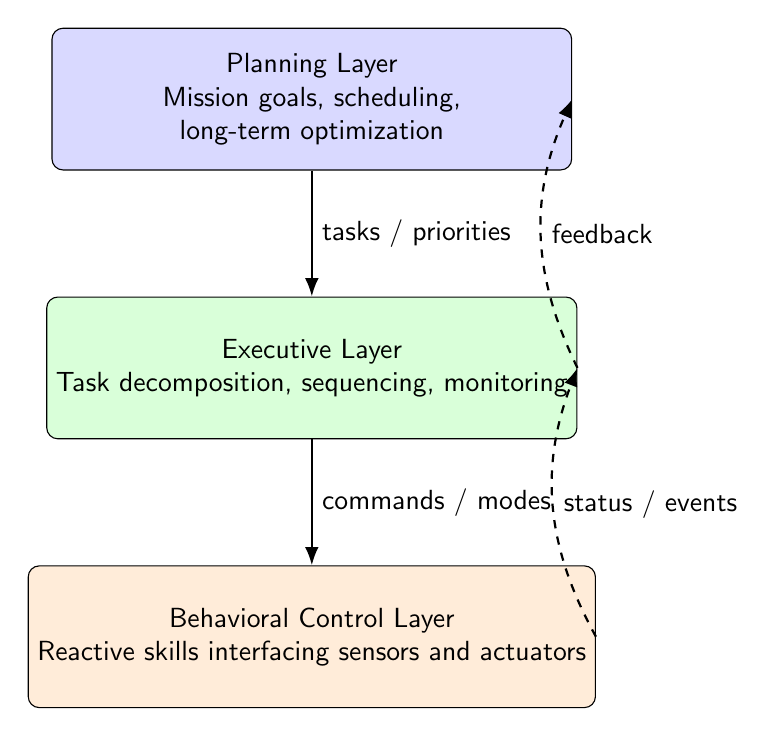
\begin{tikzpicture}[font=\sffamily,>=Latex,node distance=1.6cm]
  \tikzstyle{layer}=[draw,rounded corners=4pt,minimum width=6.6cm,minimum height=1.8cm,align=center,fill=gray!10]
  \node[layer,fill=blue!15] (planning) {Planning Layer\\Mission goals, scheduling,\\long-term optimization};
  \node[layer,fill=green!15,below=of planning] (executive) {Executive Layer\\Task decomposition,\ sequencing, monitoring};
  \node[layer,fill=orange!15,below=of executive] (behavioral) {Behavioral Control Layer\\Reactive skills interfacing\ sensors and actuators};
  \draw[->,thick] (planning) -- node[right]{tasks / priorities} (executive);
  \draw[->,thick] (executive) -- node[right]{commands / modes} (behavioral);
  \draw[->,thick,dashed,bend left=25] (behavioral.east) to node[right]{status / events} (executive.east);
  \draw[->,thick,dashed,bend left=25] (executive.east) to node[right]{feedback} (planning.east);
\end{tikzpicture}
\end{document}
